\documentclass[a4paper,12pt,ukrainian,oneside]{book}
\usepackage[T2A]{fontenc}
\usepackage[utf8]{inputenc}
\usepackage{amssymb,amsmath,amsthm}
\usepackage{vmargin}
\usepackage{setspace}
\usepackage[ukrainian]{babel}
\usepackage{tikz}
\usepackage[unicode,colorlinks]{hyperref}
\usepackage{pdfpages}
\usepackage{lecturemath}
\usetikzlibrary{patterns,positioning}

\newlength\tindent
\setlength{\tindent}{\parindent}
\setlength{\parindent}{0pt}
\renewcommand{\indent}{\hspace*{\tindent}}


\begin{document}
\tableofcontents
\numberwithin{equation}{section}
кандидат технічних наук, доцент Самойленко Олексій Васильович\\
095-781-97-79, 096-481-21-84\\
samoilenko@i.ua\\
patent.inf.ua, samoilenko.kiev.ua
\chapter{Інтелектуальна власність}
% !TeX spellcheck = uk_UA
\section{Система інтелектуальної власності}\marginpar{\framebox{01.09.2015}}
\subsection{Основні поняття та визначення}
\textbf{Право ІВ} - це право на результат творчої діяльності людини.

\textbf{ОПІВ} - об’єкт права інтелектуальної власності. \textbf{Завжди} нематеріальний.

Право ІВ має подвійну природу: 
\begin{itemize}
	\item Особисте немайнове право
	\item Майнове право
\end{itemize}

Особисте немайнове право невіддільне від автора і немає обмежень у просторі та часі. Складається з
\begin{itemize}
	\item Право людини на визнання її творцем ОПІВ
	\item Право на перешкоджання такого використання ОПІВ, яке може завдати шкоди честі чи репутації автора
	\item Інші особисті немайнові права передбачені законодавством (право оприлюднювати твір анонімно, під псевдонімом і так далі)
\end{itemize}

Майнові права віддільні від автора і мають обмеження у просторі та часі. Складаються з
\begin{itemize}
	\item Право використовувати ОПІВ у власній господарській діяльності
	\item Виключне право дозволяти використання ОПІВ іншим особам
	\item Виключне право перешкоджати неправомірному використанню ОПІВ
	\item Інші майнові права передбачені законодавством
\end{itemize}

Право на ОПІВ і право на матеріальний об’єкт в якому цей ОПІВ втілено незалежні одне від одного. 

В загальному розумінні право ІВ тримається на трьох моментах:
\begin{itemize}
	\item Авторство (хто автор)
	\item Пріоритет (хто перший)
	\item Обсяг охорони (що ми охороняємо)
\end{itemize}
\subsection{Класифікація ОПІВ}
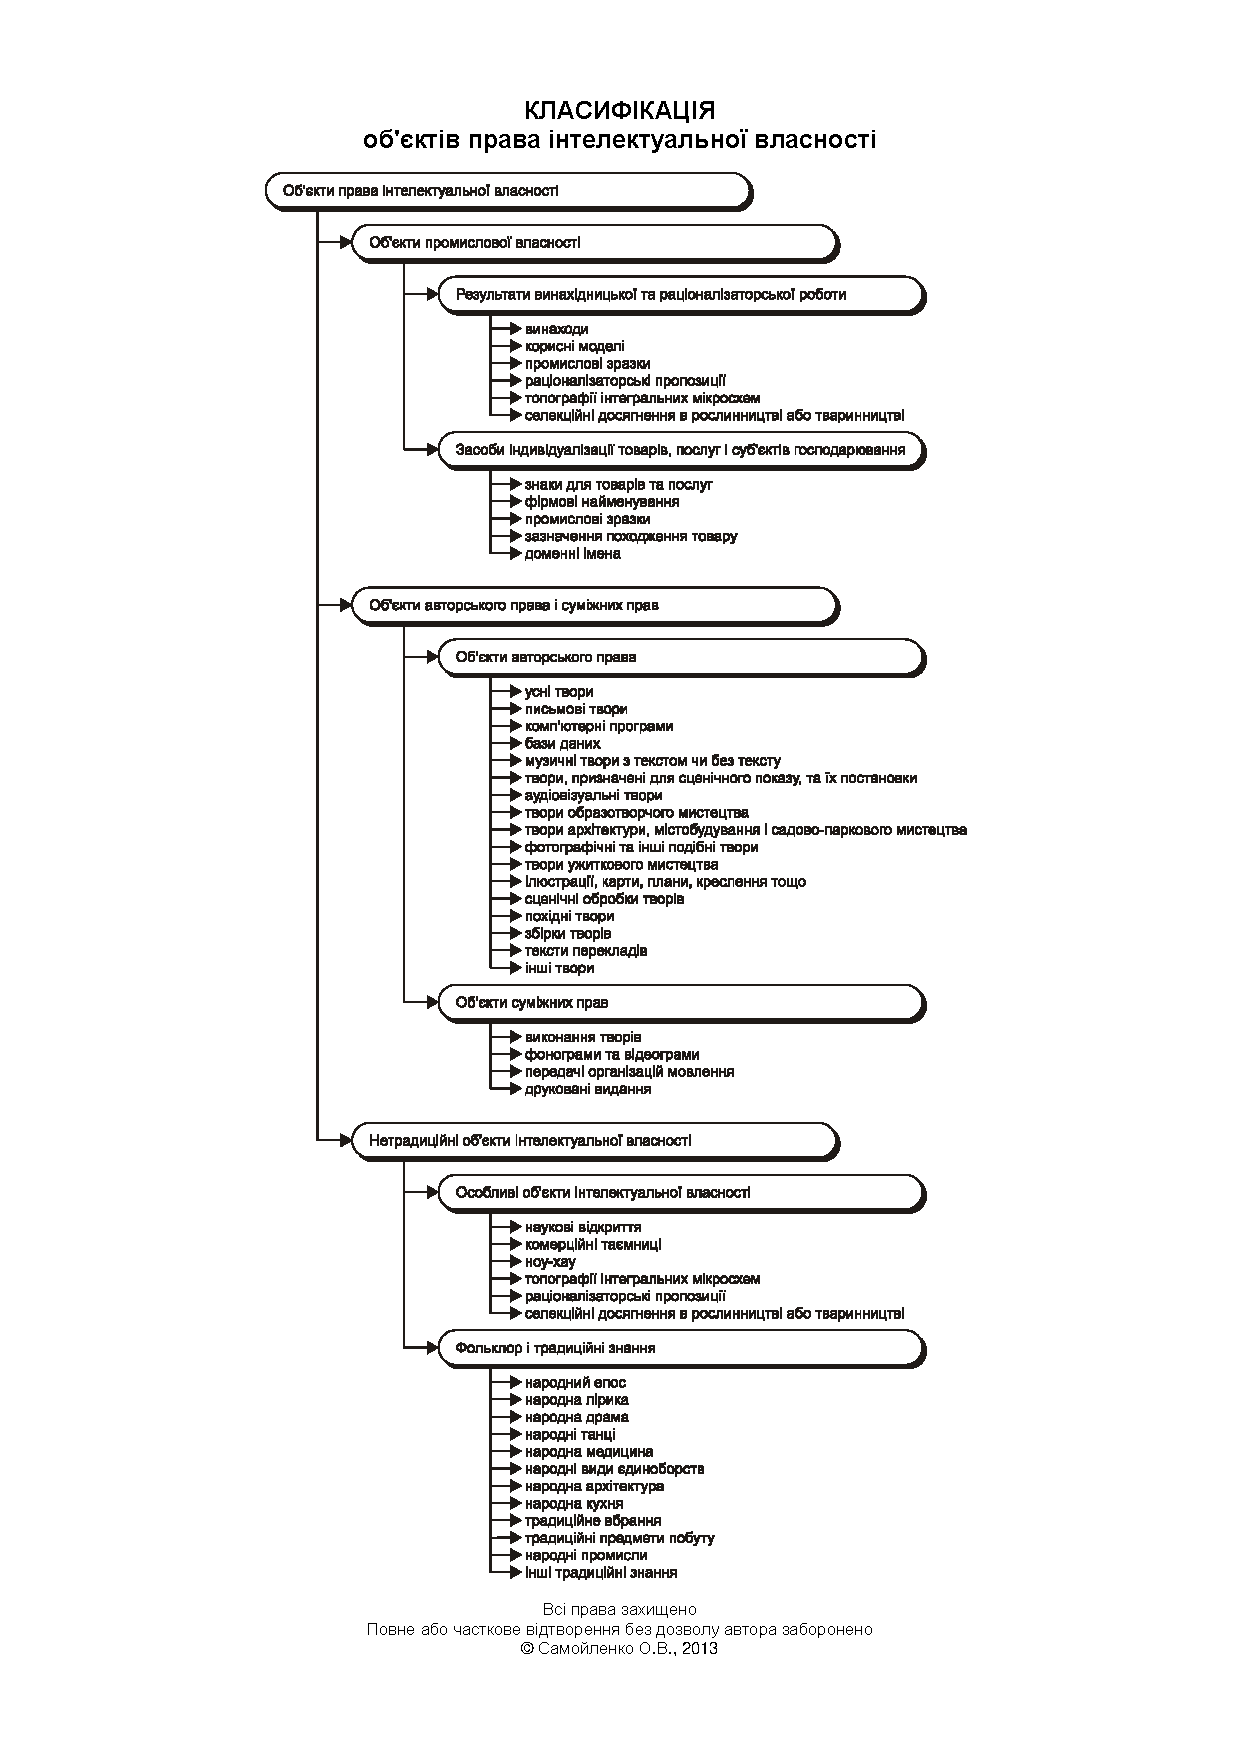
\includegraphics[scale=0.75]{opiv.pdf}
Об’єкти промислової власності названі так тому, що використовуються в основному у промисловості. Не плутати з промисловими потужностями. Головною особливістю ОПВ (об’єктів промислової власності) є те, що права на них виникають після успішного проходження ряду експертиз та виконання інших обов’язкових формальностей. 

Об’єкт суміжного права та суміжних прав. Відрізняється від ОПВ тим, що права на них виникають автоматично за фактом створення твору. І для виникнення прав не обхідно жодних формальностей.

% !TeX spellcheck = uk_UA
\subsection{Суб’єкти} 
\textbf{Суб’єктами права} можуть бути автори або інші особи, яким можуть належати майнові права на ОПІК.

\textbf{Автор} - це завжди фізична особа або група фізичних осіб. Особа автора є первинною і саме від нього походять всі майнові та немайнові права. 

Майнові права можуть належати автору, роботодавцю, покупцю, спадкоємцю, обдарованому і так далі.

Після закінчення терміну дії охоронного документа або закінчення терміну правової охорони, майнові права зникають і ОПІВ стає суспільним надбанням. Тобто, його може використовувати будь-хто, але привласнити його собі не може. 

\subsection{Законодавство у сфері ІВ}
\subsubsection{Вітчизняне законодавство}
Вітчизняне законодавство можна умовно розділити на загальне та спеціальне.  

До загального законодавства відносяться: Конституція України (4 статті), Кодекси(9 штук): по перше Цивільний кодекс (книга четверта), далі Цивільно-процесуальний кодекс, Господарський і Господарсько-процесуальний кодекс, Кримінальний і Кримінально-процесуальний, кодекс законів про працю, кодекс про адміністративні правопорушення і митний кодекс. Після кодексів йдуть закони (завантажити). Останнім рівнем є підзаконні акти.

До спеціального законодавства відносяться закони України та пов’язані з ними підзаконні акти, які стосуються охорони конкретних видів ОПІВ або подоланню конкретних проблем (наприклад, недобросовісної конкуренції). Перелік законів також на сайті.

\subsubsection{Міжнародне законодавство}

При виникненні суперечок стосовно ОПІВ між резидентом України та іноземної держави, верховенство над українським законодавством мають ті міжнародні угоди, до яких приєдналась Україна і ця держава.

Його основу становлять понад 20 міжнародних угод, приблизно дві третини яких стосуються об’єктів промислової власності, а третина про авторські права та суб’єкти прав.

Ці угоди вважаються міжнародно визнаними, адмініструє ці угоди Всесвітня організації інтелектуальної власності. ВОІВ заснована була в 1967 році на Дипломатичній конференцій в Стокгольмі. З 1974 року, ВОЇВ є однією із спеціалізованих організацій ООН. До 200 країн об’єднує.

При ній діє Всесвітня академія інтелектуальної власності. Ця академія декілька разів на рік проводить курси (безкоштовні та за свідоцтвом)

Забезпечує єдині або подібні принципи охорони ОПІВ в усіх країнах-підписантах.	

Друга група угод призначення для прискорення, спрощення і здешевлення процедури отримання охорони ОПІВ одразу в декількох країнах.

Запроваджує міжнародні класифікації об’єктів промислової власності.

\subsection{Державна система правової охорони інтелектуальної власності в Україні}
Охорона ОПІВ покладена на міністерство освіти та науки. А реалізує державну політику с сфері охорони ІВ Державна служба інтелектуальної власності. Воно ще й працює над вдосконаленням законодавства. Туди входить декілька дочірніх організацій: ДП "Український інститут інтелектуальної власності" (приймає заявки на об’єкти промислової власності, проводить експертизу і виносить рішення), ДП "Українське агентство з авторських та суміжних прав" (здійснює колективне управлення правами авторів, але заявка сюди не подається), ДП "Інтелзахист" (регулює обіг контрольних марок на ОПІВ в Україні). Біля неї крутиться купа громадських організацій. 
\chapter{Практика}
\section{Література}
\end{document} 
